\subsection{Progettazione di Dettaglio e Codifica}
Dal 2020-03-16 al 2020-04-19\\
Inizia al termine della fase di Progettazione Architetturale e finisce con la data di consegna della Revisione di Qualifica.\\
In questa fase si definisce nel dettaglio e si implementa l'architettura logica costruita nella fase di Progettazione Architetturale.

\subsubsection{Periodo 1} 
Dal 2020-03-16 al 2020-03-22
\begin{itemize}
	\item \textbf{Approfondimento delle tecnologie}: Ricerca documentazione e materiali utili per l'apprendimento delle nuove tecnologie da utilizzare per la realizzazione del prodotto finale;
	\item \textbf{Normazione}: Standardizzazione e correzione di alcune parti della documentazione e che non aderiscono completamente alle \NdP{};
	\item \textbf{Correzioni}: Correzioni di difetti notati dal committente (ove presenti) nella \glo{Technology Baseline};
	\item \textbf{Assegnazione dei ruoli di progetto}: Assegnazione dei ruoli di ciascun membro del gruppo in base alla suddivisione oraria indicata in §5.3.1;
	\item \textbf{Pianificazione delle attività}: Le attività da svolgere devono essere prima pianificate e discusse dal gruppo per garantire il \glo{way of working} sancito nelle \NdP{};
	\item \textbf{Progettazione}: Gli incrementi definiti nella sezione §3.3 vengono analizzati e vengono prodotti i diagrammi delle classi, dei package e le relazioni di dipendenza fra essi non ancora analizzati nell'Incremento 0, per poter nel successivo periodo procedere a una progettazione di dettaglio incrementale.
\end{itemize}
\paragraph{Milestone sull'ITS di GitHub}
\begin{itemize}
	\item \href{https://github.com/qb-team/Stalker-Documentazione/milestone/11}{Documentazione};
	\item \href{https://github.com/qb-team/Stalker-Backend/milestone/1}{Backend};
	\item \href{https://github.com/qb-team/Stalker-Admin/milestone/1}{Admin}.
\end{itemize}

\subsubsection{Periodo 2} 
Dal 2020-03-23 al 2020-04-08
\begin{itemize}
	\item \textbf{Implementazione della Product Baseline}: Seguendo le specifiche della \glo{Technology Baseline}, viene realizzata una prima versione stabile del prodotto, \glo{baseline} per il lavoro futuro;
	\item \textbf{Progettazione e codifica incrementale}: Seguendo gli incrementi definiti in §3.3, i requisiti da soddisfare vengono progettati e successivamente codificati. Per ogni incremento, vengono realizzati:
	\begin{itemize}
		\item diagrammi delle classi;
		\item diagrammi dei package;
		\item diagrammi di attività;
		\item diagrammi di sequenza.
	\end{itemize}
	La loro realizzazione viene svolta seguendo lo standard \glo{UML} ed è necessaria per la progettazione delle \glo{REST API}, che seguono invece lo standard \glo{OpenAPI}.
	Una volta che la progettazione di dettaglio di tutto ciò che permette di soddisfare i requisiti degli incrementi è stata completata, si può procedere alla codifica delle tre parti del prodotto software da realizzare: app, web-app, server.
	L'obiettivo del gruppo in questa fase è progettare almeno gli incrementi con i requisiti obbligatori per poter soddisfare gli \glo{stakeholder};
	\item \textbf{Verifica}: \glo{Verifiche} (tramite i test) per assicurarsi della bontà dei requisiti implementati;
	\item \textbf{Manuali}: Stesura del Manuale Utente e del Manuale Manutentore in relazione alle funzionalità di base del sistema.
\end{itemize}
\paragraph{Milestone sull'ITS di GitHub}
\begin{itemize}
	\item \href{https://github.com/qb-team/Stalker-Documentazione/milestone/12}{Documentazione};
	\item \href{https://github.com/qb-team/Stalker-Backend/milestone/2}{Backend};
	\item \href{https://github.com/qb-team/Stalker-Admin/milestone/2}{Admin}.
\end{itemize}

\subsubsection{Periodo 3}
Dal 2020-04-09 al 2020-04-12
\begin{itemize}
	\item \textbf{Primo rilascio del prodotto}: Pubblicazione del prodotto eseguibile all'interno dei \glo{repository} del gruppo;
	\item \textbf{Verifica}: \glo{Verifica} dell'andamento del team in relazione alle tempistiche e allo svolgimento dei compiti assegnati.
\end{itemize}
\paragraph{Milestone sull'ITS di GitHub}
\begin{itemize}
	\item \href{https://github.com/qb-team/Stalker-Documentazione/milestone/13}{Documentazione};
	\item \href{https://github.com/qb-team/Stalker-Backend/milestone/3}{Backend};
	\item \href{https://github.com/qb-team/Stalker-Admin/milestone/3}{Admin}.
\end{itemize}

\subsubsection{Periodo 4} 
Dal 2020-04-13 al 2020-04-19
\begin{itemize}
	\item \textbf{Consolidamento}: Ogni membro si prende del tempo per ripassare tutto il lavoro svolto e per studiare il necessario per affrontare al meglio le fasi successive;
	\item \textbf{Preparazione per la Revisione di Qualifica}: Il gruppo produce il materiale necessario da esporre alla presentazione pubblica della propria proposta.
\end{itemize}
\paragraph{Milestone sull'ITS di GitHub}
\begin{itemize}
	\item \href{https://github.com/qb-team/Stalker-Documentazione/milestone/14}{Documentazione};
	\item \href{https://github.com/qb-team/Stalker-Backend/milestone/4}{Backend};
	\item \href{https://github.com/qb-team/Stalker-Admin/milestone/4}{Admin}.
\end{itemize}

%PAGINA ORIZZONTALE
\newpage
\paperwidth=\pdfpageheight
\paperheight=\pdfpagewidth
\pdfpageheight=\paperheight
\pdfpagewidth=\paperwidth
\headwidth=\textheight

\begingroup 
\vsize=\textwidth
\hsize=\textheight

\subsubsection{Diagramma di Gantt delle attività di Progettazione di Dettaglio e Codifica}
\pagestyle{empty}
\begin{figure}[h]
	\centering
	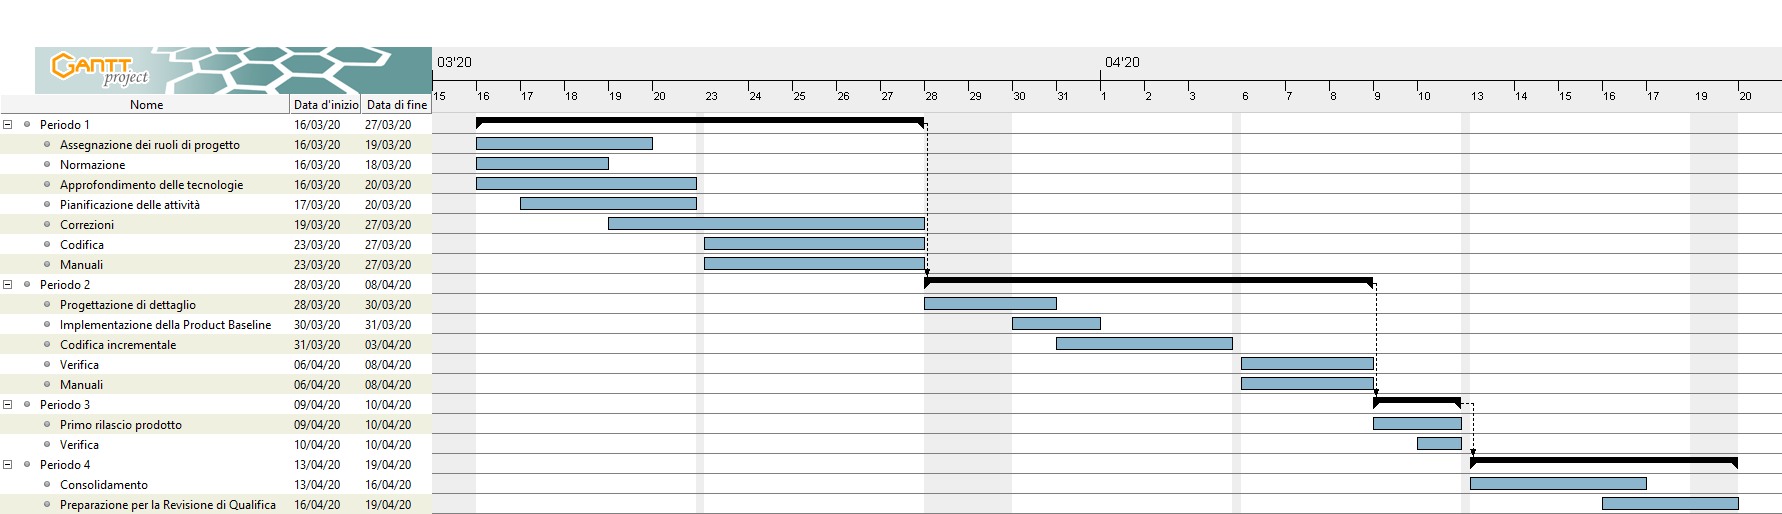
\includegraphics[height = 8cm, width = 24.5cm]{Sezioni/DiagrammiGantt/ProgettazioneDiDettaglio.png}
	\caption{Diagramma di Gantt delle attività di Progettazione di Dettaglio e Codifica}
\end{figure}

\textwidth=\hsize
\textheight=\vsize

\endgroup
\newpage
\paperwidth=\pdfpageheight
\paperheight=\pdfpagewidth
\pdfpageheight=\paperheight
\pdfpagewidth=\paperwidth
\headwidth=\textwidth